% Options for packages loaded elsewhere
\PassOptionsToPackage{unicode}{hyperref}
\PassOptionsToPackage{hyphens}{url}
%
\documentclass[
]{article}
\usepackage{amsmath,amssymb}
\usepackage{iftex}
\ifPDFTeX
  \usepackage[T1]{fontenc}
  \usepackage[utf8]{inputenc}
  \usepackage{textcomp} % provide euro and other symbols
\else % if luatex or xetex
  \usepackage{unicode-math} % this also loads fontspec
  \defaultfontfeatures{Scale=MatchLowercase}
  \defaultfontfeatures[\rmfamily]{Ligatures=TeX,Scale=1}
\fi
\usepackage{lmodern}
\ifPDFTeX\else
  % xetex/luatex font selection
\fi
% Use upquote if available, for straight quotes in verbatim environments
\IfFileExists{upquote.sty}{\usepackage{upquote}}{}
\IfFileExists{microtype.sty}{% use microtype if available
  \usepackage[]{microtype}
  \UseMicrotypeSet[protrusion]{basicmath} % disable protrusion for tt fonts
}{}
\makeatletter
\@ifundefined{KOMAClassName}{% if non-KOMA class
  \IfFileExists{parskip.sty}{%
    \usepackage{parskip}
  }{% else
    \setlength{\parindent}{0pt}
    \setlength{\parskip}{6pt plus 2pt minus 1pt}}
}{% if KOMA class
  \KOMAoptions{parskip=half}}
\makeatother
\usepackage{xcolor}
\usepackage{longtable,booktabs,array}
\usepackage{calc} % for calculating minipage widths
% Correct order of tables after \paragraph or \subparagraph
\usepackage{etoolbox}
\makeatletter
\patchcmd\longtable{\par}{\if@noskipsec\mbox{}\fi\par}{}{}
\makeatother
% Allow footnotes in longtable head/foot
\IfFileExists{footnotehyper.sty}{\usepackage{footnotehyper}}{\usepackage{footnote}}
\makesavenoteenv{longtable}
\usepackage{graphicx}
\makeatletter
\newsavebox\pandoc@box
\newcommand*\pandocbounded[1]{% scales image to fit in text height/width
  \sbox\pandoc@box{#1}%
  \Gscale@div\@tempa{\textheight}{\dimexpr\ht\pandoc@box+\dp\pandoc@box\relax}%
  \Gscale@div\@tempb{\linewidth}{\wd\pandoc@box}%
  \ifdim\@tempb\p@<\@tempa\p@\let\@tempa\@tempb\fi% select the smaller of both
  \ifdim\@tempa\p@<\p@\scalebox{\@tempa}{\usebox\pandoc@box}%
  \else\usebox{\pandoc@box}%
  \fi%
}
% Set default figure placement to htbp
\def\fps@figure{htbp}
\makeatother
\ifLuaTeX
  \usepackage{luacolor}
  \usepackage[soul]{lua-ul}
\else
  \usepackage{soul}
\fi
\setlength{\emergencystretch}{3em} % prevent overfull lines
\providecommand{\tightlist}{%
  \setlength{\itemsep}{0pt}\setlength{\parskip}{0pt}}
\setcounter{secnumdepth}{-\maxdimen} % remove section numbering
\usepackage{bookmark}
\IfFileExists{xurl.sty}{\usepackage{xurl}}{} % add URL line breaks if available
\urlstyle{same}
\hypersetup{
  hidelinks,
  pdfcreator={LaTeX via pandoc}}

\author{}
\date{}

\begin{document}

\section{\texorpdfstring{\ul{Agents}}{Agents}}\label{agents}

\section{\texorpdfstring{1. \emph{What is an
Agent?}}{1. What is an Agent?}}\label{1-what-is-an-agent}

\paragraph{Definition:}\label{definition}

\begin{itemize}
\item
  An \textbf{agent} is "anything" that can perceive its environment
  through sensors and acts upon the environment through actuators.
\end{itemize}

\pandocbounded{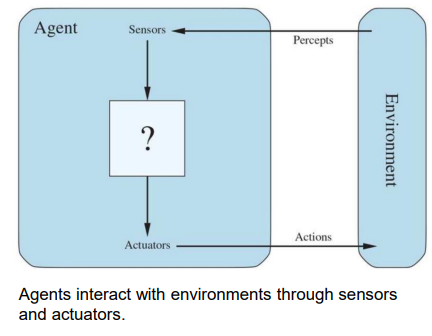
\includegraphics[keepaspectratio]{C:/Users/H3llJoY/Downloads/Documents/Third Sem Documents/Introduction to Artifical intelligence/MD/ImagesNote/image-20240704060605817.png}}

\paragraph{Key Components:}\label{key-components}

\begin{enumerate}
\def\labelenumi{\arabic{enumi}.}
\item
  \textbf{Sensors}: Devices or mechanisms that allow the agent to
  perceive or gather information from its environment.
\item
  \textbf{Actuators}: Components that enable the agent to act upon or
  influence the environment based on the information gathered.
\end{enumerate}

\paragraph{Examples and Analogies:}\label{examples-and-analogies}

\begin{enumerate}
\def\labelenumi{\arabic{enumi}.}
\item
  \textbf{Human}:

  \begin{itemize}
  \item
    \textbf{Sensors}: Eyes, ears, skin, etc., which allow humans to see,
    hear, feel, and perceive their surroundings.
  \item
    \textbf{Actuators}: Muscles and limbs that enable humans to move,
    speak, and interact with their environment.
  \end{itemize}
\item
  \textbf{Cleaning Robot}:

  \begin{itemize}
  \item
    \textbf{Sensors}: Cameras, infrared sensors, bump sensors, etc., to
    detect obstacles, dirt, and navigate the space.
  \item
    \textbf{Actuators}: Wheels, brushes, suction mechanisms, etc., to
    move around and clean the floor.
  \end{itemize}
\item
  \textbf{Software Agents}:

  \begin{itemize}
  \item
    \textbf{Sensors}: APIs, data inputs, web scrapers, etc., to gather
    information from digital environments (e.g., the internet,
    databases).
  \item
    \textbf{Actuators}: Algorithms, scripts, network requests, etc., to
    perform tasks like data processing, sending emails, or interacting
    with other software systems.
  \end{itemize}
\end{enumerate}

\begin{center}\rule{0.5\linewidth}{0.5pt}\end{center}

\section{\texorpdfstring{2. \emph{The Agent
Function}}{2. The Agent Function}}\label{2-the-agent-function}

\paragraph{Key Concepts:}\label{key-concepts}

\begin{enumerate}
\def\labelenumi{\arabic{enumi}.}
\item
  \textbf{Agent Function}:

  \begin{itemize}
  \item
    \textbf{Definition}: The agent function maps the agent's percept
    sequence to an action.
  \item
    \textbf{Percept Sequence}: The complete history of everything an
    agent has perceived so far.
  \item
    \textbf{Ideal Mapping}: Specifies the actions an agent should take
    for any given percept sequence.
  \end{itemize}
\item
  \textbf{Agent Program}:

  \begin{itemize}
  \item
    \textbf{Definition}: The implementation of the agent function.
  \item
    The agent program is the software or code that dictates how the
    agent behaves based on its percept sequence.
  \end{itemize}
\item
  \textbf{Performance Measure}:

  \begin{itemize}
  \item
    \textbf{Definition}: The effectiveness of the agent function is
    evaluated using a performance measure.
  \item
    \textbf{Purpose}: It quantifies how well the agent is performing
    with respect to the goals or objectives it is designed to achieve.
  \end{itemize}
\end{enumerate}

\pandocbounded{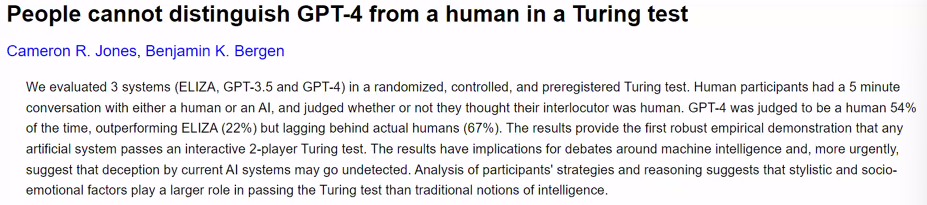
\includegraphics[keepaspectratio]{C:/Users/H3llJoY/Downloads/Documents/Third Sem Documents/Introduction to Artifical intelligence/MD/ImagesNote/image-20240624105634891.png}}

\begin{center}\rule{0.5\linewidth}{0.5pt}\end{center}

\section{\texorpdfstring{3. \emph{Good Behavior: The Concept of
Rationality}}{3. Good Behavior: The Concept of Rationality}}\label{3-good-behavior-the-concept-of-rationality}

\subsection{\texorpdfstring{\ul{Rational Agent
?}}{Rational Agent ?}}\label{rational-agent-}

\begin{itemize}
\item
  \textbf{Definition}: A rational agent is one that does the right
  thing.
\item
  Determining the Right Thing:

  \begin{itemize}
  \item
    \textbf{Performance Measure}: A criterion that evaluates the success
    of the agent\textquotesingle s actions.
  \item
    \textbf{Percept Sequence}: The complete history of what the agent
    has perceived up to the current moment.
  \item
    \textbf{Knowledge of the Environment}: Information the agent has
    about its surroundings.
  \item
    \textbf{Available Actions}: The set of actions the agent can
    perform.
  \end{itemize}
\end{itemize}

\subsection{\texorpdfstring{\ul{Performance Measures}
:}{Performance Measures :}}\label{performance-measures-}

\begin{enumerate}
\def\labelenumi{\arabic{enumi}.}
\item
  \textbf{Consequentialism}:

  \begin{itemize}
  \item
    \textbf{Definition}: Evaluating an agent's behavior based on the
    consequences of its actions.
  \item
    \textbf{Purpose}: To assess how successful the
    agent\textquotesingle s actions are in achieving its goals.
  \end{itemize}
\item
  \textbf{Examples}:

  \begin{itemize}
  \item
    Cleaning Robot :

    \begin{itemize}
    \item
      \textbf{Performance Criterion}: The cleanliness of the floor.
    \item
      Points System :

      \begin{itemize}
      \item
        Award points for each clean square at each time step.
      \item
        Deduct points for electricity consumed and noise generated.
      \end{itemize}
    \item
      \textbf{Objective}: The robot should take actions that maximize
      its overall points.
    \end{itemize}
  \end{itemize}
\item
  \textbf{Designing Performance Measures}:

  \begin{itemize}
  \item
    \textbf{Focus on Desired Outcomes}: Design performance measures
    based on the desired state of the environment, not on preconceived
    notions of how the agent should act.
  \item
    \textbf{Objective-Based}: Ensure that the performance measure aligns
    with the actual goals of the agent's operation.
  \end{itemize}
\end{enumerate}

\pandocbounded{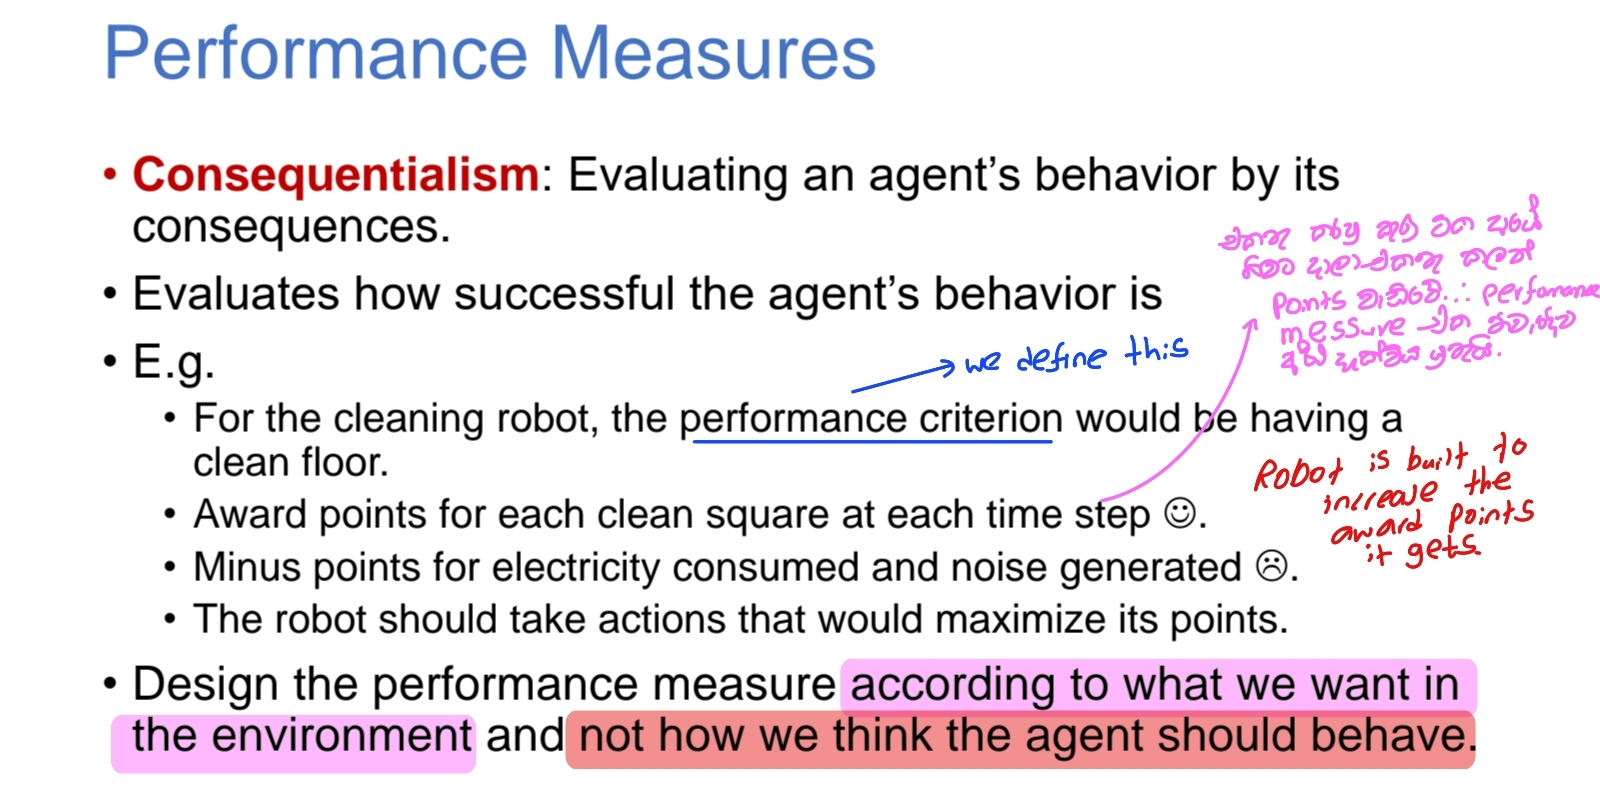
\includegraphics[keepaspectratio]{C:/Users/H3llJoY/Downloads/Documents/Third Sem Documents/Introduction to Artifical intelligence/MD/ImagesNote/image-20240704060345289.png}}

\begin{center}\rule{0.5\linewidth}{0.5pt}\end{center}

\subsection{\texorpdfstring{\ul{Definition of Rational
Agent}}{Definition of Rational Agent}}\label{definition-of-rational-agent}

\paragraph{Key Concepts :}\label{key-concepts-}

\begin{enumerate}
\def\labelenumi{\arabic{enumi}.}
\item
  \textbf{Rational Agent}:

  \begin{itemize}
  \item
    For each possible percept sequence, a rational agent selects an
    action expected to maximize its performance measure.The choice is
    based on the evidence provided by the percept sequence and the
    built-in knowledge of the agent.
  \end{itemize}
\item
  \textbf{Example }:

  \begin{itemize}
  \item
    Crossing the Road:

    \begin{itemize}
    \item
      An agent that can only look sideways checks that the road is clear
      before crossing.
    \item
      If something falls from above and crushes the agent, it is still
      considered rational.
    \item
      \textbf{Reason}: The agent acted based on its perceptual
      capabilities and available knowledge, which did not include the
      ability to look up.
    \end{itemize}
  \end{itemize}
\end{enumerate}

\paragraph{Rational Agent Example : Vacuum-Cleaner
Agent}\label{rational-agent-example--vacuum-cleaner-agent}

Performance Measure:

\begin{itemize}
\item
  Awards one point for each clean square at each time step over a
  lifetime of 1000-time steps.
\end{itemize}

Environment:

\begin{itemize}
\item
  \textbf{Geography}: Known beforehand.
\item
  \textbf{Dirt Distribution and Initial Location}: Unknown.
\item
  \textbf{Behavior of Clean Squares}: They remain clean after being
  cleaned.
\end{itemize}

Actions:

\begin{itemize}
\item
  \textbf{Right (Move Right)}: Moves the agent one square to the right
  unless it is at the boundary.
\item
  \textbf{Left (Move Left)}: Moves the agent one square to the left
  unless it is at the boundary.
\item
  \textbf{Suck (Clean)}: Cleans the current square if it contains dirt.
\end{itemize}

Perception:

\begin{itemize}
\item
  The agent correctly perceives its current location and whether that
  location contains dirt.
\end{itemize}

\subsection{\texorpdfstring{\ul{Building Rational
Agents}}{Building Rational Agents}}\label{building-rational-agents}

\paragraph{Key Concepts:}\label{key-concepts-2}

\begin{enumerate}
\def\labelenumi{\arabic{enumi}.}
\item
  \textbf{AI and Rational Agents}:

  \begin{itemize}
  \item
    \textbf{Objective}: AI focuses on building rational agents that
    always do the right thing.
  \end{itemize}
\item
  \textbf{Types of Rationality}:

  \begin{itemize}
  \item
    Perfect Rationality :

    \begin{itemize}
    \item
      Assumes the agent has complete knowledge of everything.
    \item
      Always takes the action that maximizes its utility.
    \end{itemize}
  \item
    Bounded Rationality :

    \begin{itemize}
    \item
      Proposed by Herbert Simon in 1958.
    \item
      Agents are limited by the information they have.
    \item
      Use approximate methods to handle tasks, similar to how the human
      mind operates.
    \end{itemize}
  \end{itemize}
\end{enumerate}

\paragraph{Rationality:}\label{rationality}

\begin{enumerate}
\def\labelenumi{\arabic{enumi}.}
\item
  \textbf{Rational Action}:

  \begin{itemize}
  \item
    The action that maximizes the expected value of the performance
    measure given the percept sequence to date.
  \end{itemize}
\item
  \textbf{Questions About Rational Action}:

  \begin{itemize}
  \item
    Is it the best action? :

    \begin{itemize}
    \item
      \texttt{Rational\ action\ is\ considered\ the\ best\ given\ the\ information\ available\ to\ the\ agent\ at\ the\ time\ of\ the\ decision}.
    \end{itemize}
  \item
    Is it optimal? :

    \begin{itemize}
    \item
      \texttt{Rational\ action\ is\ not\ always\ optimal\ in\ the\ sense\ of\ perfect\ rationality.\ It\ is\ optimal\ within\ the\ bounds\ of\ the\ agent\textquotesingle{}s\ knowledge\ and\ computational\ limits.}
    \end{itemize}
  \end{itemize}
\end{enumerate}

\begin{center}\rule{0.5\linewidth}{0.5pt}\end{center}

\subsection{\texorpdfstring{\ul{Omniscience, Learning, and Autonomy in
AI}}{Omniscience, Learning, and Autonomy in AI}}\label{omniscience-learning-and-autonomy-in-ai}

\begin{itemize}
\item
  \textbf{Omniscience}

  \begin{itemize}
  \item
    The agent knows the actual outcome of its actions and acts
    accordingly.
  \item
    Ideal but not practically achievable; complete knowledge is often
    unrealizable.
  \end{itemize}

  \textbf{Rationality}

  \begin{itemize}
  \item
    The agent maximizes expected outcomes based on available
    information.
  \item
    Decision-making depends on the percept sequence to date, not
    requiring omniscience.
  \item
    This requires a rational agent to:

    \begin{itemize}
    \item
      Gather information
    \item
      Learn from perceptions
    \end{itemize}
  \end{itemize}

  \textbf{Autonomy}

  \begin{itemize}
  \item
    More Autonomous:

    \begin{itemize}
    \item
      Agent\textquotesingle s actions rely on learning from its own
      experiences gathered through sensors.
    \end{itemize}
  \item
    Less Autonomous:

    \begin{itemize}
    \item
      Agent\textquotesingle s actions depend more on knowledge of the
      environment provided by designers.
    \end{itemize}
  \end{itemize}
\end{itemize}

\begin{center}\rule{0.5\linewidth}{0.5pt}\end{center}

\section{\texorpdfstring{4. \emph{The Task
Environment}}{4. The Task Environment}}\label{4-the-task-environment}

\subsection{Task Environment
Components}\label{task-environment-components}

\begin{enumerate}
\def\labelenumi{\arabic{enumi}.}
\item
  \textbf{Defines the problems to which the rational agents attempt to
  provide solutions:}

  \begin{itemize}
  \item
    The task environment specifies the goals or problems that the agents
    are designed to address. This could include tasks like navigating a
    maze, playing chess, or interpreting natural language.
  \end{itemize}
\item
  \textbf{Consists of PEAS:}

  \begin{itemize}
  \item
    PEAS stands for:

    \begin{itemize}
    \item
      \textbf{Performance Measure:} Defines what constitutes success in
      the task. It\textquotesingle s the criteria used to evaluate the
      agent\textquotesingle s performance.
    \item
      \textbf{Environment:} Describes the context or setting in which
      the agent operates, including physical aspects and other entities
      present.
    \item
      \textbf{Actuators:} Specifies how the agent interacts with the
      environment, such as motors or outputs for performing actions.
    \item
      \textbf{Sensors:} How the agent perceives or gathers information
      from its environment, such as cameras, microphones, or other
      sensors.
    \end{itemize}
  \end{itemize}
\end{enumerate}

\subsubsection{Designing an Agent}\label{designing-an-agent}

\begin{itemize}
\item
  Specifying the task environment fully:

  This involves detailing each component of PEAS:

  \begin{itemize}
  \item
    \textbf{Performance Measure:} Clearly define what the agent is
    supposed to achieve or optimize.
  \item
    \textbf{Environment:} Describe the conditions, entities, and
    constraints in which the agent operates.
  \item
    \textbf{Actuators:} Specify the mechanisms or methods through which
    the agent can affect the environment.
  \item
    \textbf{Sensors:} Outline how the agent perceives or gathers
    information from its environment to make decisions.
  \end{itemize}

  \pandocbounded{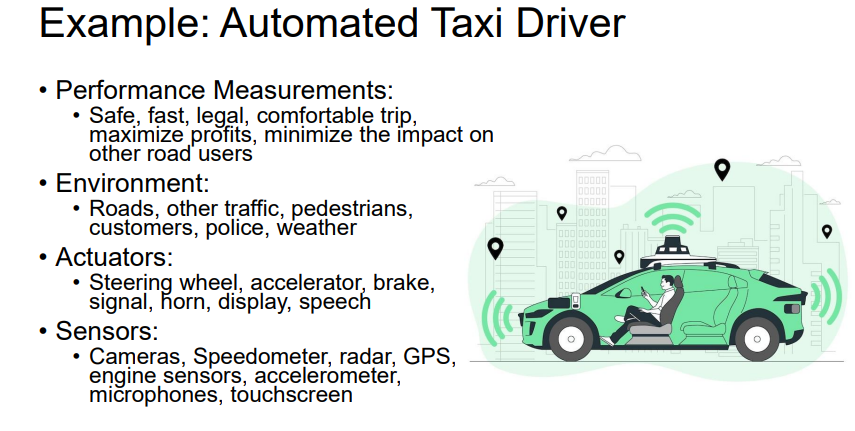
\includegraphics[keepaspectratio]{C:/Users/H3llJoY/Downloads/Documents/Third Sem Documents/Introduction to Artifical intelligence/MD/ImagesNote/image-20240704065752106.png}}
\end{itemize}

\subsection{Importance of Task Environment
Specification}\label{importance-of-task-environment-specification}

\begin{itemize}
\item
  \textbf{Foundation for agent design:} By thoroughly defining the task
  environment, you provide the foundational requirements and constraints
  that guide the design of the agent. This ensures that the agent is
  appropriately equipped to achieve its objectives effectively.
\end{itemize}

\pandocbounded{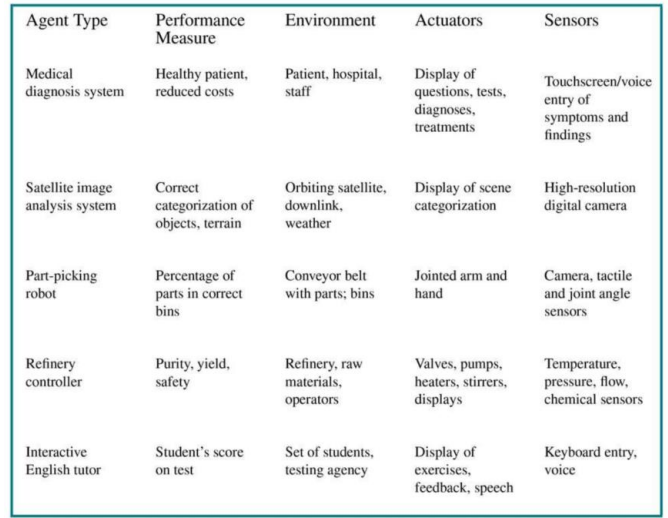
\includegraphics[keepaspectratio]{C:/Users/H3llJoY/Downloads/Documents/Third Sem Documents/Introduction to Artifical intelligence/MD/ImagesNote/image-20240704065837964.png}}

\begin{center}\rule{0.5\linewidth}{0.5pt}\end{center}

\subsection{Properties of Task
Environments}\label{properties-of-task-environments}

Observed from the agent\textquotesingle s point of View.

\subsubsection{\texorpdfstring{\textbf{1. Fully Observable vs. Partially
Observable:}}{1. Fully Observable vs. Partially Observable:}}\label{1-fully-observable-vs-partially-observable}

\begin{itemize}
\item
  Fully Observable: The agent\textquotesingle s sensors provide complete
  access to the environment\textquotesingle s state at any given time.

  \begin{itemize}
  \item
    Fully observable environments are convenient.
  \end{itemize}
\item
  Partially Observable: The agent\textquotesingle s sensors may provide
  incomplete or noisy information about the
  environment\textquotesingle s state.

  \begin{itemize}
  \item
    Example:

    \begin{itemize}
    \item
      A vacuum cleaner with a local dirt sensor can\textquotesingle t
      perceive dirt in other square.
    \item
      A vacuum agent with only a local dirt sensor cannot tell whether
      there is dirt in other squares.
    \item
      An automated taxi cannot see what other drivers are thinking.
    \end{itemize}
  \end{itemize}
\item
  \pandocbounded{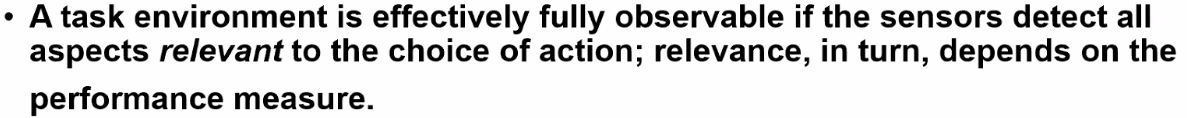
\includegraphics[keepaspectratio]{C:/Users/H3llJoY/Downloads/Documents/Third Sem Documents/Introduction to Artifical intelligence/MD/ImagesNote/image-20240704073616176.png}}
\end{itemize}

\subsubsection{\texorpdfstring{\textbf{2. Single-Agent vs.
Multi-Agent:}}{2. Single-Agent vs. Multi-Agent:}}\label{2-single-agent-vs-multi-agent}

\begin{itemize}
\item
  Single-Agent:

  An environment where there is only one agent affecting the state.

  \begin{itemize}
  \item
    Example: A crossword puzzle solver.
  \end{itemize}
\item
  Multi-Agent:

  Multiple agents interact within the environment, affecting each
  other\textquotesingle s states.

  \begin{itemize}
  \item
    Example: Agents playing a game of chess where each
    agent\textquotesingle s moves impact the overall state.
  \end{itemize}
\item
  \pandocbounded{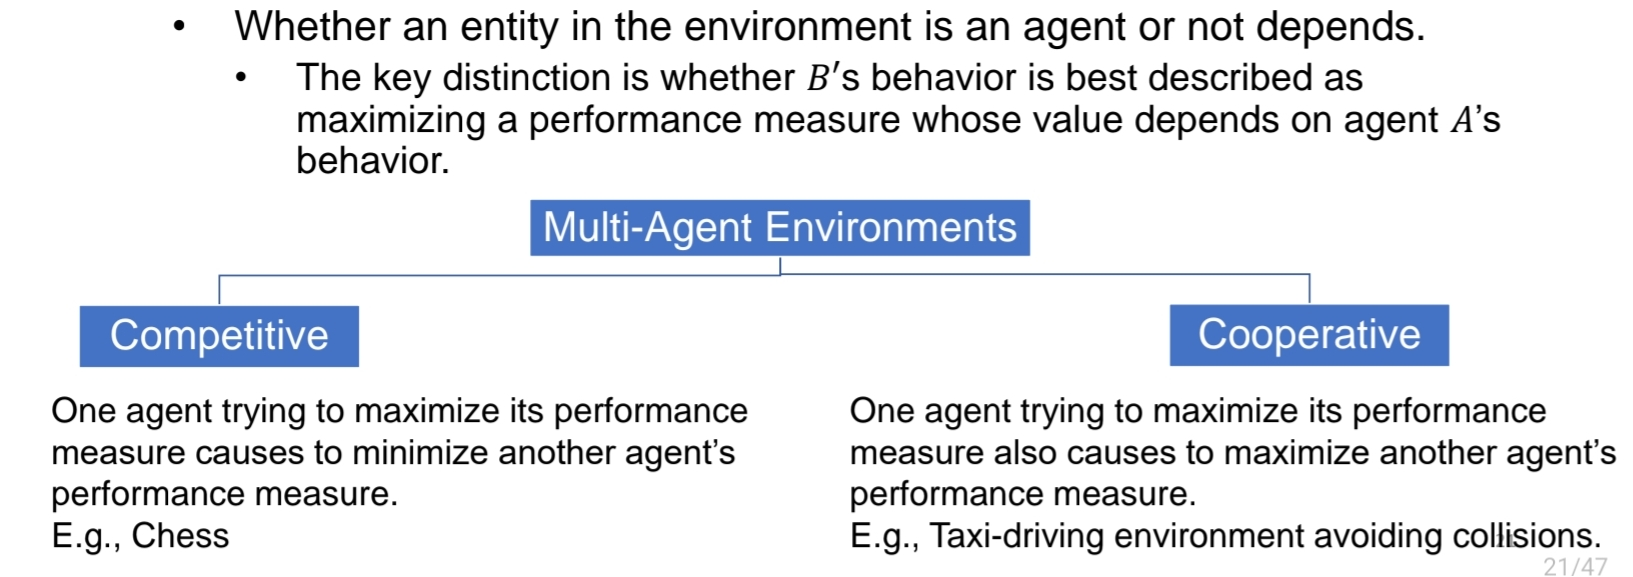
\includegraphics[keepaspectratio]{C:/Users/H3llJoY/Downloads/Documents/Third Sem Documents/Introduction to Artifical intelligence/MD/ImagesNote/image-20240704073728922.png}}
\end{itemize}

\subsubsection{\texorpdfstring{\textbf{3. Deterministic vs.
Nondeterministic vs.
Stochastic:}}{3. Deterministic vs. Nondeterministic vs. Stochastic:}}\label{3-deterministic-vs-nondeterministic-vs-stochastic}

\begin{itemize}
\item
  Deterministic:

  The next state of the environment is completely determined by the
  current state and actions taken. There is no randomness
  involved.\texttt{Given\ the\ same\ initial\ conditions,\ a\ deterministic\ system\ will\ always\ produce\ the\ same\ result}.

  \begin{itemize}
  \item
    Example: Simple physical systems with known rules / Chess
  \end{itemize}
\item
  Nondeterministic:

  The next state may not be fully determined by the current state and
  actions due to randomness or unknown factors.

  \begin{itemize}
  \item
    Example: Taxi driving where traffic conditions can vary
    unpredictably.
  \end{itemize}
\item
  Stochastic:

  Environment changes explicitly incorporate probabilities.

  \begin{itemize}
  \item
    Example: Weather forecasting where the chance of rain is stated as a
    probability.
  \item
    \begin{quote}
    \textbf{Deterministic} and \textbf{Nondeterministic} describe
    different types of systems or processes based on the predictability
    of their outcomes:

    \subsubsection{\texorpdfstring{\textbf{Deterministic}:}{Deterministic:}}\label{deterministic}

    \begin{itemize}
    \item
      \textbf{Predictability}: The outcome is entirely predictable.
    \item
      \textbf{Definition}: In a deterministic system, given the current
      state and the actions taken, the next state is fully determined
      with no randomness involved. If you repeat the process with the
      same initial conditions, you will always get the same result.
    \item
      \textbf{Example}: A simple calculator performing addition. If you
      input \texttt{2\ +\ 3}, it will always output \texttt{5},
      regardless of how many times you perform the operation.
    \end{itemize}

    \subsubsection{\texorpdfstring{\textbf{Nondeterministic}:}{Nondeterministic:}}\label{nondeterministic}

    \begin{itemize}
    \item
      \textbf{Unpredictability}: The outcome may vary even with the same
      initial conditions.
    \item
      \textbf{Definition}: In a nondeterministic system, the next state
      is not fully determined by the current state and actions. There
      may be randomness, unknown factors, or multiple possible outcomes
      for the same initial conditions.
    \item
      \textbf{Example}: A taxi ride in a city. Even if you start from
      the same location and follow the same route, the time it takes to
      reach your destination can vary due to traffic conditions,
      roadblocks, or other unpredictable factors.
    \end{itemize}
    \end{quote}
  \end{itemize}
\end{itemize}

\subsubsection{\texorpdfstring{\textbf{4. Episodic vs.
Sequential:}}{4. Episodic vs. Sequential:}}\label{4-episodic-vs-sequential}

\begin{itemize}
\item
  Episodic: One action is not influenced to the next action

  Each interaction or episode is self-contained and independent of
  previous episodes.

  \begin{itemize}
  \item
    Example: Inspecting items on an assembly line where each inspection
    is isolated.
  \end{itemize}
\item
  Sequential:

  Actions and decisions in the current episode affect future episodes.

  \begin{itemize}
  \item
    Example: Chess, where each move influences subsequent moves.
  \end{itemize}

  \begin{quote}
  \subsubsection{\texorpdfstring{\textbf{Deterministic}:}{Deterministic:}}\label{deterministic-2}

  \begin{itemize}
  \item
    \textbf{Focus}: The predictability of the outcome.
  \item
    \textbf{Definition}: A system is deterministic if the next state is
    entirely determined by the current state and the actions taken, with
    no randomness involved. If you know the current state and the
    actions, you can predict the next state with certainty.
  \item
    \textbf{Example}: A simple mathematical function like
    \texttt{f(x)\ =\ 2x} is deterministic. Given the same input
    \texttt{x}, it will always produce the same output.
  \end{itemize}

  \subsubsection{\texorpdfstring{\textbf{Sequential}:}{Sequential:}}\label{sequential}

  \begin{itemize}
  \item
    \textbf{Focus}: The dependency of current actions on previous
    actions.
  \item
    \textbf{Definition}: A sequential system is one where the current
    action affects future states or outcomes. In other words, the
    decisions or actions in one step have consequences that influence
    what happens next.
  \item
    \textbf{Example}: Playing chess is sequential because each move you
    make affects the future possibilities and strategies in the game.
  \end{itemize}

  \subsubsection{\texorpdfstring{\textbf{Key
  Difference}:}{Key Difference:}}\label{key-difference}

  \begin{itemize}
  \item
    \textbf{Deterministic} refers to the certainty of outcomes based on
    current conditions and actions, with no randomness.
  \item
    \textbf{Sequential} refers to the dependency of actions, where what
    happens now influences what happens next.
  \end{itemize}
  \end{quote}
\end{itemize}

\subsubsection{\texorpdfstring{\textbf{5. Dynamic vs.
Static:}}{5. Dynamic vs. Static:}}\label{5-dynamic-vs-static}

\begin{itemize}
\item
  Dynamic:

  The environment can change while the agent is making decisions.

  \begin{itemize}
  \item
    Example: Real-time strategy games where opponents\textquotesingle{}
    moves affect the game state. / Taxi driving
  \end{itemize}
\item
  Static:

  The environment remains unchanged while the agent deliberates.

  \begin{itemize}
  \item
    Example: Solving static puzzles like crossword puzzles.
  \end{itemize}
\end{itemize}

\subsubsection{\texorpdfstring{\textbf{6. Discrete vs.
Continuous:}}{6. Discrete vs. Continuous:}}\label{6-discrete-vs-continuous}

\begin{itemize}
\item
  Discrete:

  States, time, percepts, and actions are clearly defined and discrete.

  \begin{itemize}
  \item
    Example: Chess, where moves are discrete and finite.
  \end{itemize}
\item
  Continuous:

  States, time, percepts, and actions exist on a continuous scale.

  \begin{itemize}
  \item
    Example: Taxi driving, where movements and actions are continuous in
    both space and time.
  \end{itemize}
\end{itemize}

These properties help in categorizing and understanding different types
of environments agents may operate in, guiding how agents are designed
and how they interact effectively within their environments.

\subparagraph{examples}\label{examples}

\pandocbounded{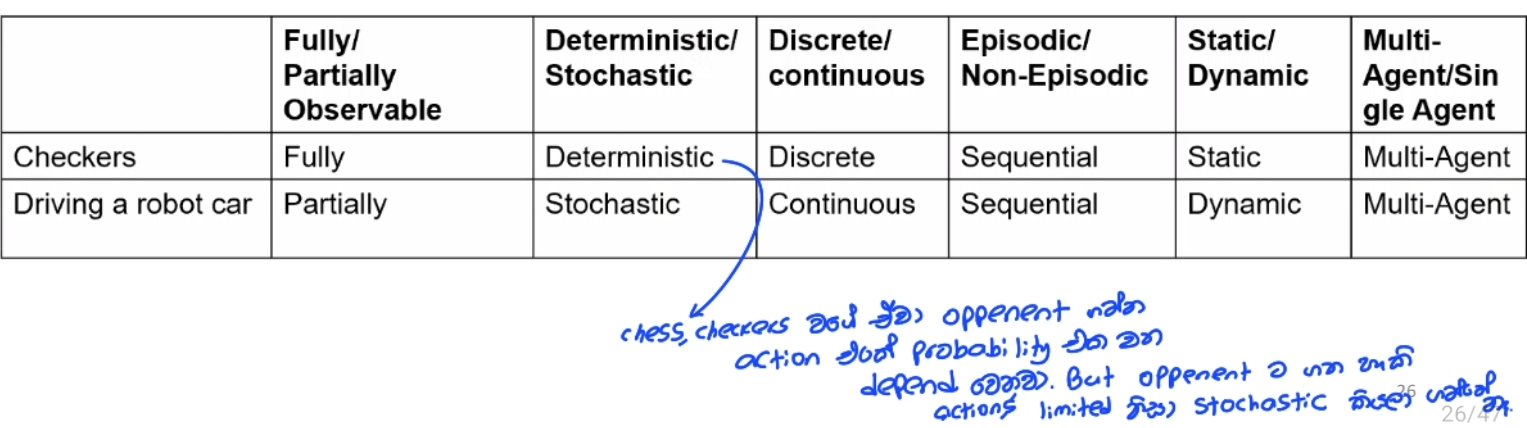
\includegraphics[keepaspectratio]{C:/Users/H3llJoY/Downloads/Documents/Third Sem Documents/Introduction to Artifical intelligence/MD/ImagesNote/image-20240704074602448.png}}

\pandocbounded{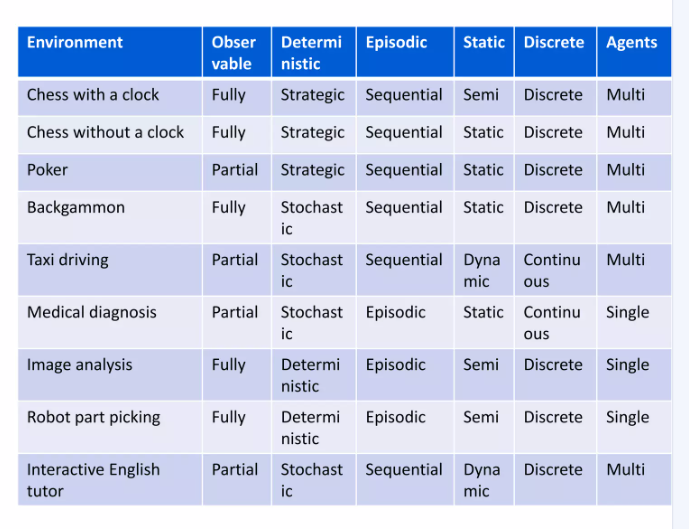
\includegraphics[keepaspectratio]{C:/Users/H3llJoY/Downloads/Documents/Third Sem Documents/Introduction to Artifical intelligence/MD/ImagesNote/image-20240704074747936.png}}

\paragraph{Summary}\label{summary}

\begin{longtable}[]{@{}
  >{\raggedright\arraybackslash}p{(\linewidth - 4\tabcolsep) * \real{0.3333}}
  >{\raggedright\arraybackslash}p{(\linewidth - 4\tabcolsep) * \real{0.3333}}
  >{\raggedright\arraybackslash}p{(\linewidth - 4\tabcolsep) * \real{0.3333}}@{}}
\toprule\noalign{}
Property & Description & Examples \\
\midrule\noalign{}
\endhead
\bottomrule\noalign{}
\endlastfoot
\textbf{Observability} & \vtop{\hbox{\strut Fully Observable:
Agent\textquotesingle s sensors provide complete state
information.}\hbox{\strut Partially Observable: Agent\textquotesingle s
sensors provide incomplete or noisy state information.}} & Vacuum
cleaner (local dirt sensor) vs. automated taxi (traffic conditions). \\
\textbf{Single-Agent vs. Multi-Agent} & \vtop{\hbox{\strut Single-Agent:
Only one agent affecting the environment.}\hbox{\strut Multi-Agent:
Multiple agents interacting, influencing each other\textquotesingle s
states.}} & Crossword puzzle solver vs. chess players. \\
\textbf{Determinism} & \vtop{\hbox{\strut Deterministic: Next state
determined by current state and actions.}\hbox{\strut Nondeterministic:
Next state may not be fully determined by current state and actions.}} &
Simple physics simulation vs. taxi driving (traffic
unpredictability). \\
\textbf{Stochasticity} & \vtop{\hbox{\strut Deterministic: No
probabilities involved.}\hbox{\strut Stochastic: Environment changes
involve explicit probabilities.}} & Weather forecasting (probability of
rain) vs. deterministic processes. \\
\textbf{Episodic vs. Sequential} & \vtop{\hbox{\strut Episodic: Actions
and experiences are isolated episodes.}\hbox{\strut Sequential: Actions
affect subsequent actions and outcomes.}} & Inspecting items on an
assembly line vs. playing chess. \\
\textbf{Dynamic vs. Static} & \vtop{\hbox{\strut Dynamic: Environment
can change while agent makes decisions.}\hbox{\strut Static: Environment
remains unchanged while agent deliberates.}} & Real-time strategy games
vs. crossword puzzles. \\
\textbf{Discrete vs. Continuous} & \vtop{\hbox{\strut Discrete: States,
time, percepts, and actions are clearly defined and
finite.}\hbox{\strut Continuous: States, time, percepts, and actions
exist on a continuous scale.}} & Chess (discrete moves) vs. taxi driving
(continuous movement). \\
\end{longtable}

\begin{center}\rule{0.5\linewidth}{0.5pt}\end{center}

\section{\texorpdfstring{5.\emph{The structure of
Agents}}{5.The structure of Agents}}\label{5the-structure-of-agents}

\begin{enumerate}
\def\labelenumi{\arabic{enumi}.}
\item
  \textbf{Agent Program:}

  \begin{itemize}
  \item
    The agent program is responsible for determining the actions of the
    agent based on its percepts.
  \item
    It implements the agent function, which is essentially a mapping
    from percepts (the inputs the agent receives from its environment)
    to actions (the outputs or responses the agent performs).
  \item
    The agent program can be thought of as the "brain" of the agent,
    containing the logic and decision-making processes.
  \end{itemize}
\item
  \textbf{Agent Architecture:}

  \begin{itemize}
  \item
    The agent architecture refers to the physical or virtual computing
    device on which the agent program runs.
  \item
    It includes sensors and actuators, which are the mechanisms through
    which the agent interacts with its environment.

    \begin{itemize}
    \item
      \textbf{Sensors}: Devices that gather information from the
      environment and provide percepts to the agent program.
    \item
      \textbf{Actuators}: Devices that carry out the actions decided by
      the agent program.
    \end{itemize}
  \item
    The architecture ensures that percepts from the sensors are made
    available to the agent program, runs the program, and sends the
    program's action choices to the actuators.
  \end{itemize}
\end{enumerate}

In summary, an agent can be defined by the combination of its
architecture and program:

\[Agent=Architecture+Program\]

\pandocbounded{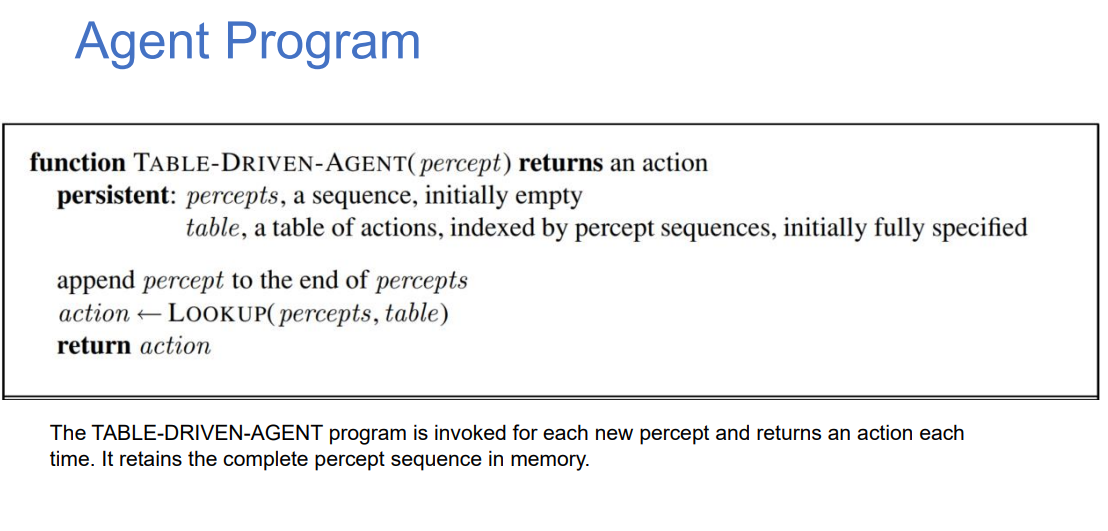
\includegraphics[keepaspectratio]{C:/Users/H3llJoY/Downloads/Documents/Third Sem Documents/Introduction to Artifical intelligence/MD/ImagesNote/image-20240714142621280.png}}

\section{\texorpdfstring{6.\emph{Agent program
types}}{6.Agent program types}}\label{6agent-program-types}

\pandocbounded{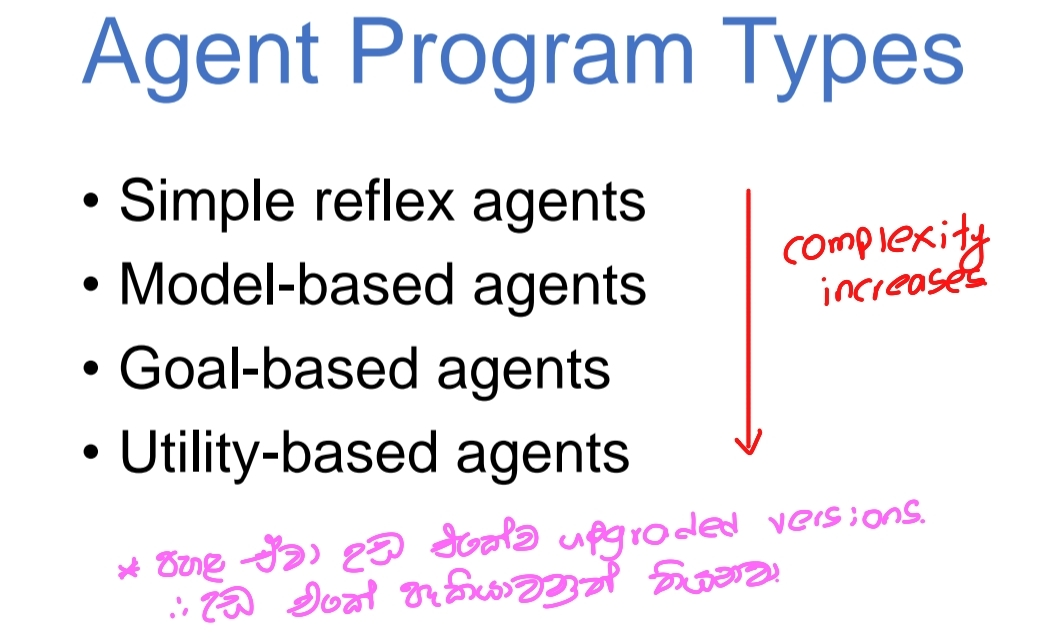
\includegraphics[keepaspectratio]{C:/Users/H3llJoY/Downloads/Documents/Third Sem Documents/Introduction to Artifical intelligence/MD/ImagesNote/image-20240714143033106.png}}

\subsection{\texorpdfstring{\ul{1.Simple Reflex
Agents}}{1.Simple Reflex Agents}}\label{1simple-reflex-agents}

Simple reflex agents act solely based on the current percept, ignoring
the rest of the percept history. \textbf{\ul{They select actions based
on a condition-action rule (if-then rules)}}, making them the simplest
form of agents.

\textbf{Characteristics:}

\begin{itemize}
\item
  React to the environment without considering the past.
\item
  Use condition-action rules to determine the action.
\item
  Suitable for simple environments with well-defined rules.
\end{itemize}

Problems with Simple reflex agents are :

\begin{itemize}
\item
  Very limited intelligence.
\item
  No knowledge of non-perceptual parts of the state.
\item
  Usually too big to generate and store.
\item
  If there occurs any change in the environment, then the collection of
  rules needs to be updated.
\end{itemize}

\textbf{Example:} A thermostat that turns on the heater if the
temperature drops below a certain threshold.

\pandocbounded{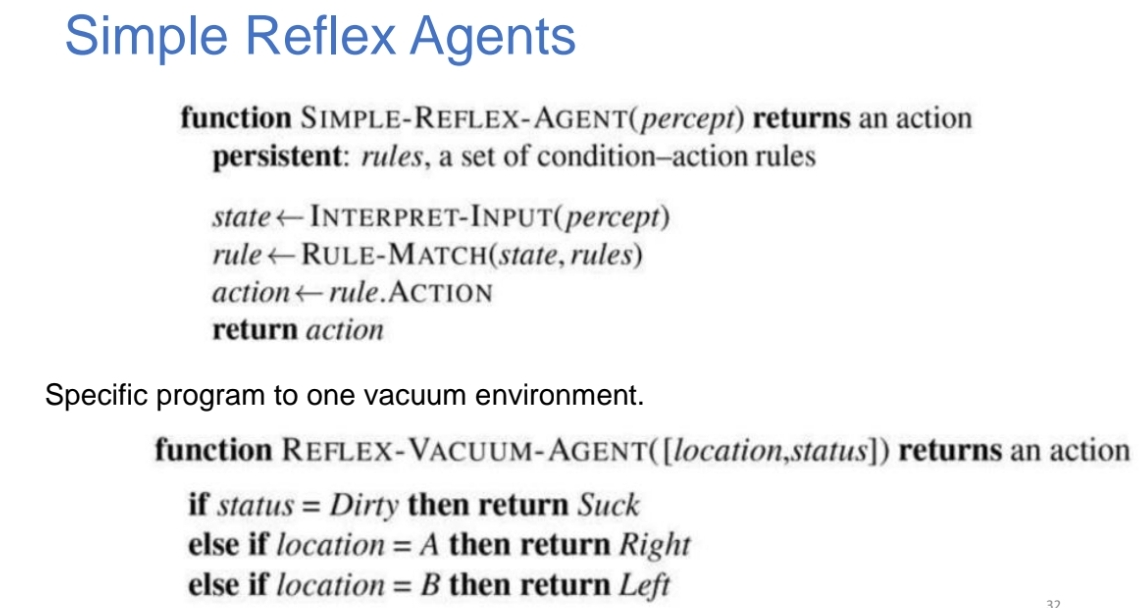
\includegraphics[keepaspectratio]{C:/Users/H3llJoY/Downloads/Documents/Third Sem Documents/Introduction to Artifical intelligence/MD/ImagesNote/image-20240714143956225.png}}

\pandocbounded{\includegraphics[keepaspectratio]{https://media.geeksforgeeks.org/wp-content/cdn-uploads/ai3-1.png}}

\emph{Simple Reflex Agents}

\subsection{\texorpdfstring{\ul{2.}\ul{Model based Reflex
Agents}}{2.Model based Reflex Agents}}\label{2model-based-reflex-agents}

Model-based reflex agents maintain an internal state to make decisions
based on the history of their percepts. This internal state is essential
for operating in partially observable environments, where not all
necessary information is available at any given time.

\ul{Key Features}

\begin{enumerate}
\def\labelenumi{\arabic{enumi}.}
\item
  \textbf{Maintains an Internal State}:

  \begin{itemize}
  \item
    \textbf{Depends on Percept History}: The internal state is updated
    based on the agent\textquotesingle s percepts over time.
  \item
    \texttt{Useful\ in\ Partially\ Observable\ Environments}: Helps the
    agent keep track of information that is not immediately perceptible.
  \end{itemize}
\item
  \textbf{Tracks Perception History}:

  \begin{itemize}
  \item
    The agent records the history of its perceptions to inform future
    actions.
  \end{itemize}
\item
  \textbf{Examples}:

  \begin{itemize}
  \item
    \textbf{Crossing the Road}: When an agent needs to cross the road,
    it will look right and then left. While looking left, it remembers
    what it saw on the right.
  \item
    \textbf{Applying Brakes}: When the vehicle in front brakes, the
    agent applies brakes based on the previous frame from the camera.
  \item
    \textbf{Changing Lanes}: The agent keeps track of where other cars
    are to make safe lane changes.
  \end{itemize}
\end{enumerate}

\ul{Maintaining the Internal State}

To maintain the internal state, the agent needs to store \ul{two kinds
of knowledge}:

\begin{enumerate}
\def\labelenumi{\arabic{enumi}.}
\item
  \textbf{Transition Model of the World}: \textbf{How the World Works}

  \emph{1.\textbf{\ul{Effects of the Agent's Actions}}}: Understanding
  how the agent\textquotesingle s actions affect the world.

  When the agent turns the steering wheel clockwise,the car turns to the
  right

  \emph{2.\textbf{\ul{World Evolution}}}: Knowledge of how the world
  changes independently of the agent's actions.

  When it\textquotesingle s raining , the car\textquotesingle s cameras
  can get wet
\item
  \textbf{Sensor Model}:

  \textbf{Reflecting World State in Percepts}: Understanding how the
  state of the world is represented in the agent's sensors.

  \pandocbounded{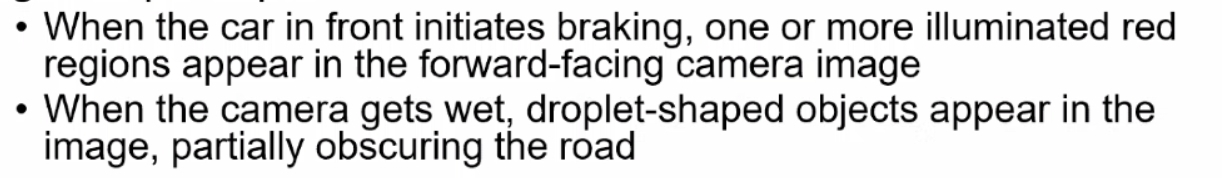
\includegraphics[keepaspectratio]{C:/Users/H3llJoY/Downloads/Documents/Third Sem Documents/Introduction to Artifical intelligence/MD/ImagesNote/image-20240714150354615.png}}
\end{enumerate}

\ul{How to Maintain the Internal State}

\begin{enumerate}
\def\labelenumi{\arabic{enumi}.}
\item
  \textbf{Update Mechanism}:

  \begin{itemize}
  \item
    \textbf{Observe}: The agent receives a percept from the environment.
  \item
    \textbf{Update State}: The agent updates its internal state based on
    the new percept and its transition model.
  \item
    \textbf{Decision Making}: The agent uses its updated internal state
    to decide the next action.
  \end{itemize}
\item
  \textbf{Example Process} in Crossing the Road:

  \begin{enumerate}
  \def\labelenumii{\arabic{enumii}.}
  \item
    \textbf{Look Right}: The agent observes the right side.
  \item
    \textbf{Update State}: It updates its internal state with the
    information about the right side.
  \item
    \textbf{Look Left}: The agent then observes the left side.
  \item
    \textbf{Update State}: It combines this new information with the
    previously stored information about the right side to decide when it
    is safe to cross.
  \end{enumerate}
\item
  \textbf{Example Process in Vehicles}:

  \begin{itemize}
  \item
    Applying Brakes:

    \begin{enumerate}
    \def\labelenumii{\arabic{enumii}.}
    \item
      \textbf{Observe}: The agent perceives that the vehicle in front is
      braking.
    \item
      \textbf{Update State}: It updates its internal state with this
      information.
    \item
      \textbf{Decide}: Based on the internal state, the agent decides to
      apply brakes.
    \end{enumerate}
  \item
    Changing Lanes:

    \begin{enumerate}
    \def\labelenumii{\arabic{enumii}.}
    \item
      \textbf{Observe}: The agent perceives the positions of surrounding
      cars.
    \item
      \textbf{Update State}: It updates its internal state with this
      spatial information.
    \item
      \textbf{Decide}: The agent uses this updated state to decide
      whether it is safe to change lanes.
    \end{enumerate}
  \end{itemize}
\end{enumerate}

\pandocbounded{\includegraphics[keepaspectratio]{https://media.geeksforgeeks.org/wp-content/uploads/art1.png}}

\emph{Model-Based Reflex Agents}

\begin{center}\rule{0.5\linewidth}{0.5pt}\end{center}

\subsection{\texorpdfstring{\ul{3.Goal based
Agents}}{3.Goal based Agents}}\label{3goal-based-agents}

Goal-based agents act to achieve specific goals. \ul{They use the
internal state to make decisions that move them closer to their goals}.
These agents consider the future consequences of their actions, leading
to more complex behaviors than reflex agents.

\textbf{Characteristics:}

\begin{itemize}
\item
  Act to achieve defined goals.
\item
  Use search and planning to decide on actions.
\item
  Can handle more complex environments and objectives.
\item
  More flexible than reflex agents\\
  • Changing the goal will change the actions appropriately. E.g., Robot
  Taxi drive
\end{itemize}

\pandocbounded{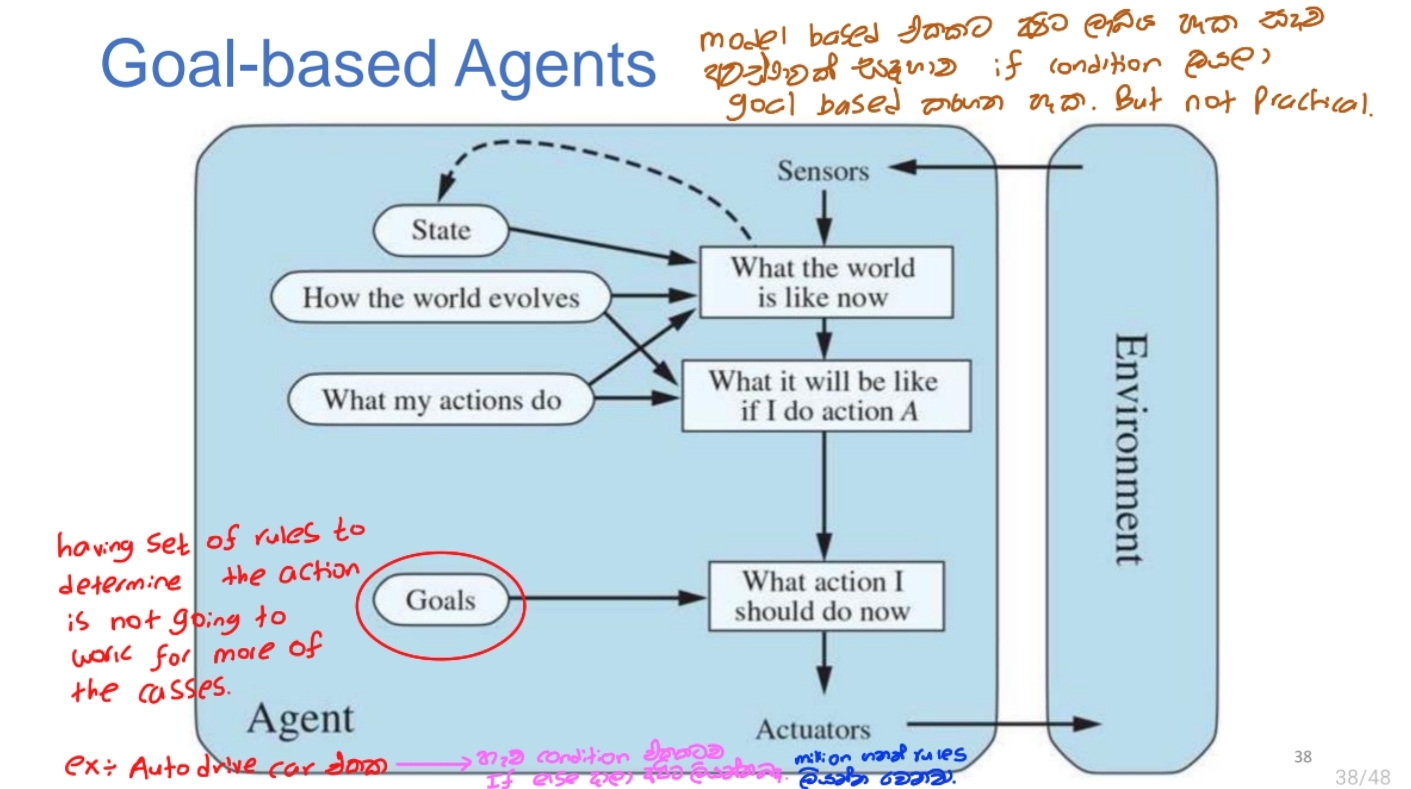
\includegraphics[keepaspectratio]{C:/Users/H3llJoY/Downloads/Documents/Third Sem Documents/Introduction to Artifical intelligence/MD/ImagesNote/image-20240714161021699.png}}

\textbf{Example:} 1. A chess-playing program that decides its moves
based on the goal of checkmating the opponent.

2. Robot car • Goal: Customers Destination (Say Ratmalana)

• Actions: at a junction, turn left/right/go straight

\subsection{\texorpdfstring{\ul{4.Utillity based
Agents}}{4.Utillity based Agents}}\label{4utillity-based-agents}

\begin{enumerate}
\def\labelenumi{\arabic{enumi}.}
\item
  \textbf{Utility Function:}

  \begin{itemize}
  \item
    A utility function is a mathematical representation that maps a
    state or a sequence of states onto a real number, indicating the
    degree of happiness or satisfaction associated with those states.
  \item
    This function helps the agent evaluate different potential outcomes
    or states, allowing it to choose the most desirable one.
  \end{itemize}
\item
  \textbf{Degree of Happiness:}

  \begin{itemize}
  \item
    The utility function quantifies how desirable a particular state is,
    describing the degree of happiness or satisfaction the agent derives
    from that state.
  \item
    Higher utility values represent more preferred states, guiding the
    agent toward decisions that maximize its overall happiness or
    satisfaction.

    \pandocbounded{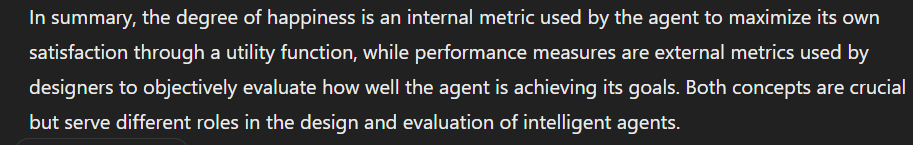
\includegraphics[keepaspectratio]{C:/Users/H3llJoY/Downloads/Documents/Third Sem Documents/Introduction to Artifical intelligence/MD/ImagesNote/image-20240714162426509.png}}
  \end{itemize}
\item
  \textbf{Use Cases:}

  \begin{itemize}
  \item
    Utility functions are particularly useful in situations where simple
    goal-based approaches are inadequate.
  \item
    They help in scenarios where there are multiple conflicting goals or
    where a single goal does not sufficiently capture the agent's
    objectives.
  \end{itemize}
\item
  \textbf{Handling Conflicting Goals:}

  \begin{itemize}
  \item
    In real-world applications, agents often face conflicting goals.
  \item
    \begin{quote}
    \texttt{For\ example,\ a\ taxi\ driver\ must\ balance\ speed\ and\ safety.}-meh
    state through yaddi kochchr happyda balala happy wadima eka
    thoranawa
    \end{quote}
  \item
    The utility function allows the agent to specify a tradeoff between
    these conflicting goals, enabling it to make decisions that
    appropriately balance these competing interests.
  \end{itemize}
\item
  \textbf{Choosing the Best Fit:}

  \begin{itemize}
  \item
    Utility-based agents are designed to choose the best fit out of many
    options by evaluating the utility of each option.
  \item
    For instance, a taxi driver might have multiple routes or actions
    available to reach the same destination. The utility function helps
    determine which route is the best based on factors like time,
    safety, fuel efficiency, and customer satisfaction.
  \end{itemize}
\end{enumerate}

Example: Taxi Driver

A utility-based agent in the context of a taxi driver would work as
follows:

\begin{itemize}
\item
  \textbf{Multiple Routes/Actions:} The taxi driver has several possible
  routes to take to reach a destination.
\item
  \textbf{Utility Evaluation:} Each route is evaluated based on a
  utility function that considers factors such as travel time, traffic
  conditions, safety, and passenger comfort.
\item
  \textbf{Best Decision:} The route with the highest utility value is
  chosen, ensuring that the driver takes the most efficient and
  satisfactory path given the current conditions and priorities.
\end{itemize}

\pandocbounded{\includegraphics[keepaspectratio]{https://media.geeksforgeeks.org/wp-content/uploads/art3.png}}

\emph{Utility-Based Agents}

\subsection{\texorpdfstring{\ul{5.Learning
Agents}}{5.Learning Agents}}\label{5learning-agents}

\pandocbounded{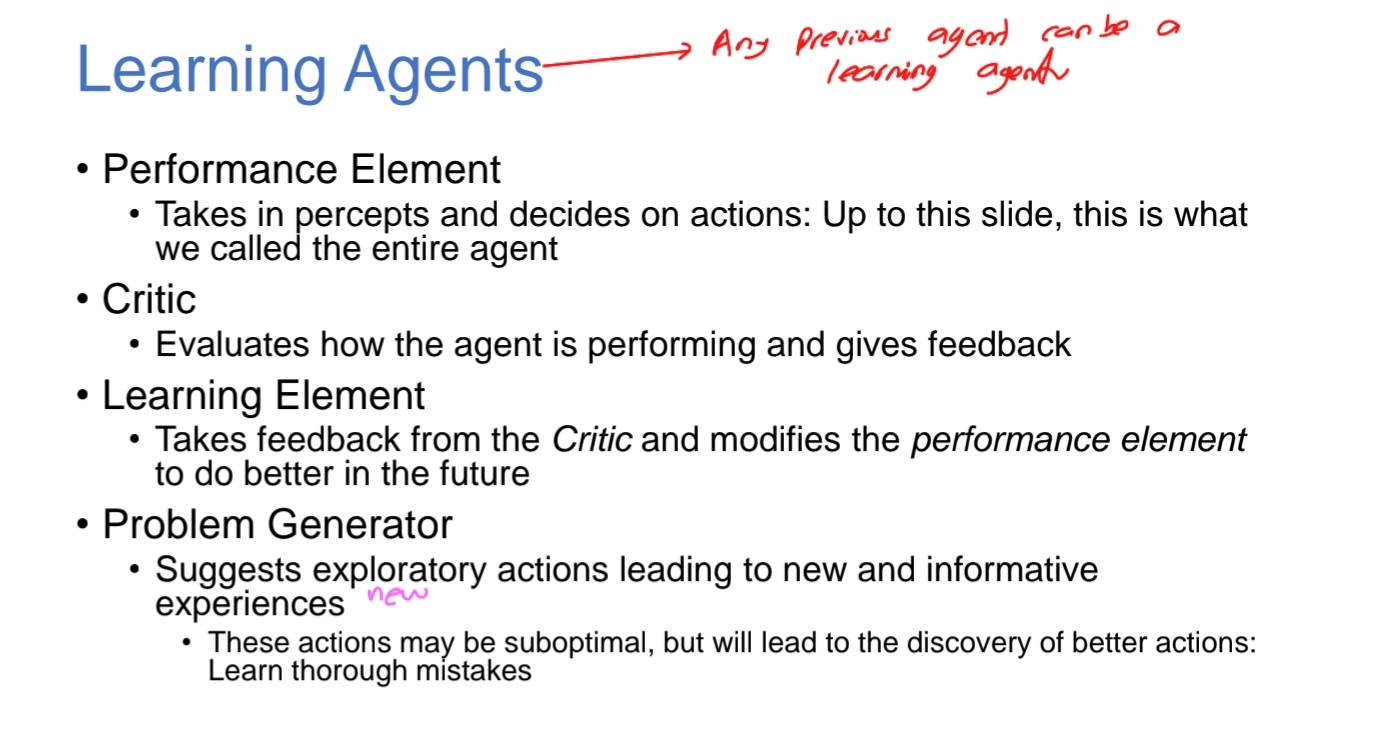
\includegraphics[keepaspectratio]{C:/Users/H3llJoY/Downloads/Documents/Third Sem Documents/Introduction to Artifical intelligence/MD/ImagesNote/image-20240714165203806.png}}

\pandocbounded{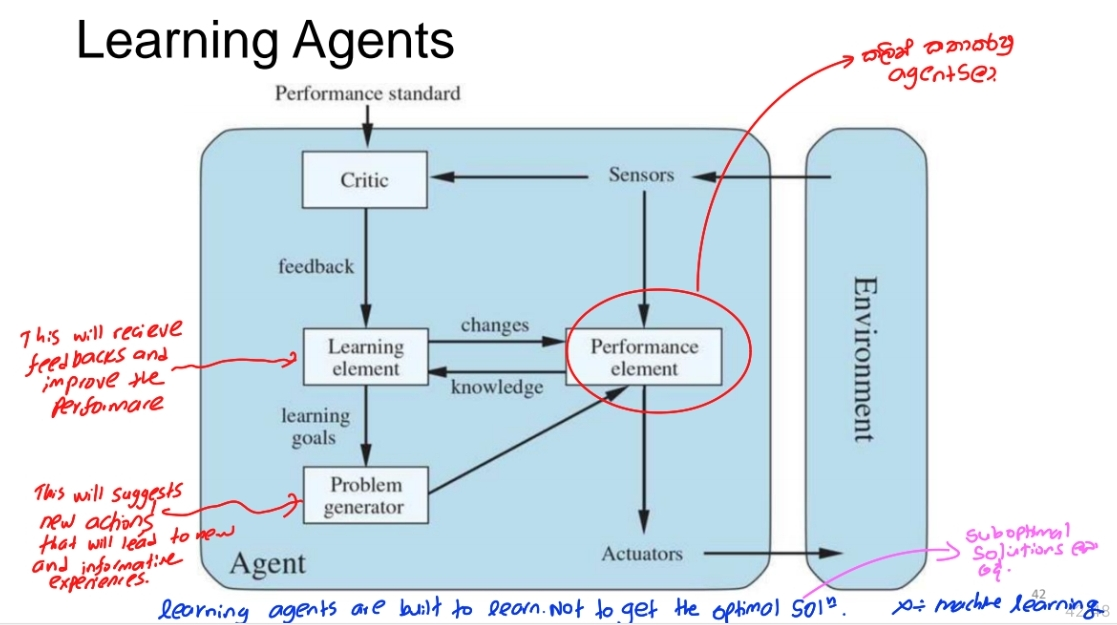
\includegraphics[keepaspectratio]{C:/Users/H3llJoY/Downloads/Documents/Third Sem Documents/Introduction to Artifical intelligence/MD/ImagesNote/image-20240714165239868.png}}

\begin{center}\rule{0.5\linewidth}{0.5pt}\end{center}

\section{\texorpdfstring{7.\emph{Components of Agent Programs
Work}}{7.Components of Agent Programs Work}}\label{7components-of-agent-programs--work}

\pandocbounded{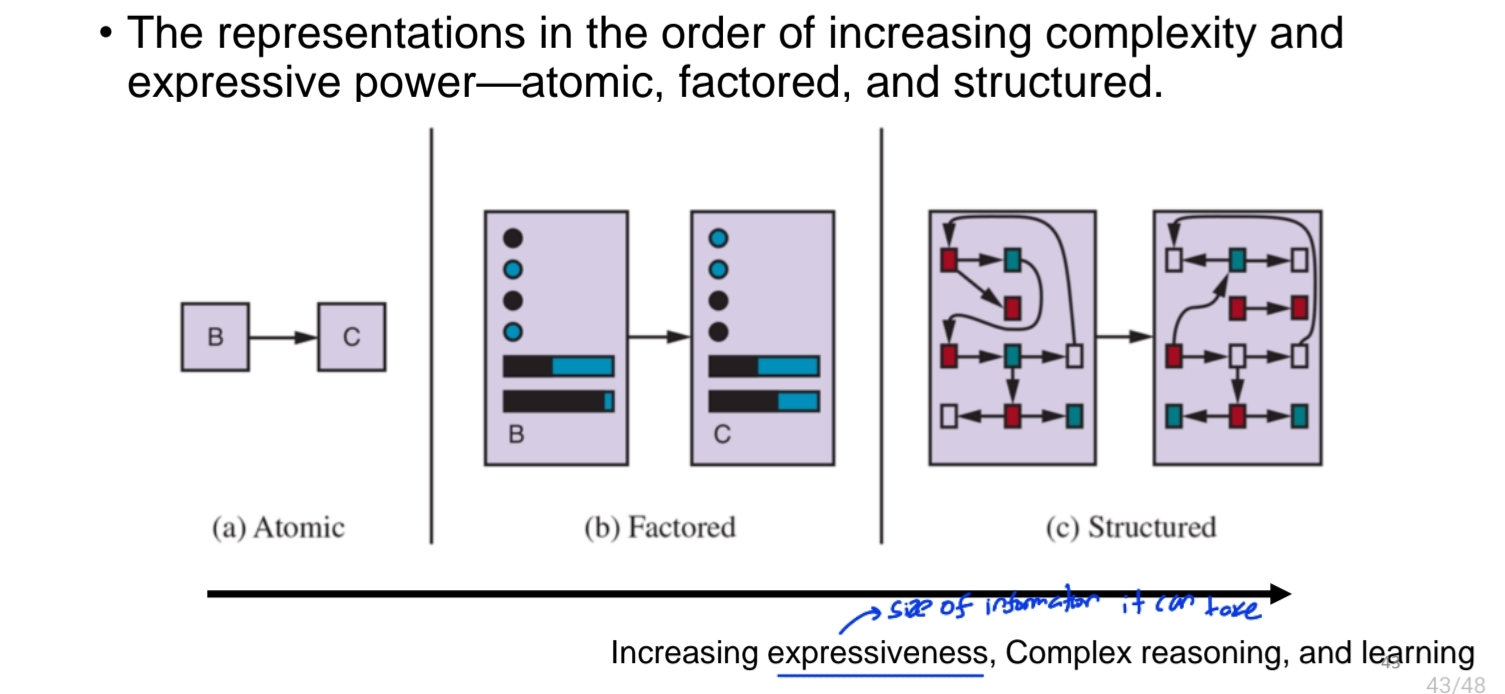
\includegraphics[keepaspectratio]{C:/Users/H3llJoY/Downloads/Documents/Third Sem Documents/Introduction to Artifical intelligence/MD/ImagesNote/image-20240714165836406.png}}

Agent programs vary in \ul{complexity and expressive power} depending on
the type of representation they use. These representations can be
broadly categorized as atomic, factored, and structured. Here's an
overview of each type:

\paragraph{\texorpdfstring{\ul{1. Atomic
Representation}}{1. Atomic Representation}}\label{1-atomic-representation}

\textbf{Definition:}

\begin{itemize}
\item
  The simplest form of representation where each state of the world is
  treated as a unique, indivisible entity.
\end{itemize}

\textbf{Components:}

\begin{itemize}
\item
  \textbf{States:} Represented as atomic symbols with no internal
  structure.
\item
  \textbf{Actions:} Defined as transitions between states.
\item
  \textbf{Percepts:} Mapped directly to states without any internal
  detail.
\end{itemize}

\textbf{Advantages:}

\begin{itemize}
\item
  Simplicity and ease of implementation.
\item
  Suitable for small problem spaces where states and actions are
  limited.
\end{itemize}

\textbf{Disadvantages:}

\begin{itemize}
\item
  Lack of detail and expressiveness.
\item
  Scalability issues as the number of states increases exponentially
  with complexity.
\end{itemize}

\textbf{Example:}

\begin{itemize}
\item
  In a maze-solving agent, each position in the maze might be
  represented as an atomic state.
\end{itemize}

\paragraph{\texorpdfstring{\ul{2. Factored
Representation}}{2. Factored Representation}}\label{2-factored-representation}

\textbf{Definition:}

\begin{itemize}
\item
  States are represented as a collection of variables, each with its own
  value, allowing for more detailed and nuanced descriptions of the
  world.
\end{itemize}

\pandocbounded{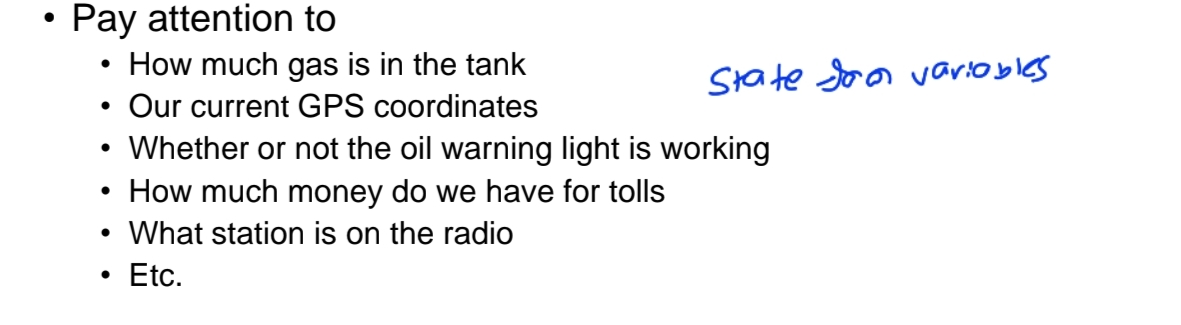
\includegraphics[keepaspectratio]{C:/Users/H3llJoY/Downloads/Documents/Third Sem Documents/Introduction to Artifical intelligence/MD/ImagesNote/image-20240714170908115.png}}

\begin{itemize}
\item
  Two different factored states can share some attributes. ( such as
  being at some GPS location)
\end{itemize}

\textbf{Components:}

\begin{itemize}
\item
  \textbf{States:} Defined by a set of variables (factors) and their
  values.
\item
  \textbf{Actions:} Defined as operations that change the values of the
  state variables.
\item
  \textbf{Percepts:} Provide information about the values of specific
  variables.
\end{itemize}

\textbf{Advantages:}

\begin{itemize}
\item
  More expressive than atomic representations.
\item
  Easier to manage and manipulate states as the number of variables
  increases.
\end{itemize}

\textbf{Disadvantages:}

\begin{itemize}
\item
  Increased complexity compared to atomic representations.
\item
  May still be challenging to handle very large state spaces.
\end{itemize}

\textbf{Example:}

\begin{itemize}
\item
  In a robotic vacuum cleaner, the state could be represented by
  variables such as position, battery level, and dirt detection.
\end{itemize}

\paragraph{\texorpdfstring{\ul{3. Structured
Representation}}{3. Structured Representation}}\label{3-structured-representation}

\textbf{Definition:}

\begin{itemize}
\item
  The most complex form, where states and actions are represented using
  relational or logical structures, allowing for detailed descriptions
  and reasoning about the world.
\end{itemize}

\textbf{Components:}

\begin{itemize}
\item
  \textbf{States:} Represented using structured objects, relations, and
  functions.
\item
  \textbf{Actions:} Defined in terms of changes to the relationships
  between objects.
\item
  \textbf{Percepts:} Provide detailed information about objects and
  their relationships.
\end{itemize}

\textbf{Advantages:}

\begin{itemize}
\item
  Highly expressive, capable of capturing complex relationships and
  dependencies.
\item
  Suitable for sophisticated reasoning and problem-solving tasks.
\end{itemize}

\textbf{Disadvantages:}

\begin{itemize}
\item
  High computational complexity.
\item
  Requires advanced algorithms for processing and reasoning.
\end{itemize}

\textbf{Example:}

\begin{itemize}
\item
  In an autonomous car, the state could be represented by a detailed map
  with objects like other vehicles, pedestrians, and traffic signals,
  along with their relationships and interactions.
\end{itemize}

\subsubsection{Summary Table}\label{summary-table}

\begin{longtable}[]{@{}llll@{}}
\toprule\noalign{}
\textbf{Aspect} & \textbf{Atomic Representation} & \textbf{Factored
Representation} & \textbf{Structured Representation} \\
\midrule\noalign{}
\endhead
\bottomrule\noalign{}
\endlastfoot
\textbf{Definition} & States as unique, indivisible entities & States as
sets of variables with values & States as structured objects and
relations \\
\textbf{State Complexity} & Simple, indivisible & Moderately complex,
with variable values & Highly complex, with detailed structures and
relations \\
\textbf{Action Definition} & Transitions between atomic states &
Operations changing variable values & Changes to relationships between
structured objects \\
\textbf{Percept Handling} & Direct mapping to states & Information about
variable values & Detailed information about objects and relations \\
\textbf{Advantages} & Simplicity, ease of implementation & More
expressive, manageable variable states & Highly expressive, suitable for
complex reasoning \\
\textbf{Disadvantages} & Limited detail, scalability issues & Increased
complexity, still challenging for large states & High computational
complexity, advanced algorithms needed \\
\textbf{Example} & Maze-solving agent (positions as atomic states) &
Robotic vacuum cleaner (position, battery, dirt) & Autonomous car (map
with vehicles, pedestrians) \\
\end{longtable}

These different levels of representation allow agents to handle a wide
range of complexities and expressiveness in their environments, from
simple tasks with limited state spaces to complex scenarios requiring
sophisticated reasoning.

\end{document}
